\documentclass[a4paper,14pt,oneside]{extreport}

\usepackage{fontspec}
\setmainfont{Times New Roman}
\setmonofont{Courier New}
\newfontfamily\cyrillicfonttt{Courier New}
\usepackage{unicode-math}
\setmathfont{STIX Two Math}
\usepackage{polyglossia}
\setdefaultlanguage{russian}
\setotherlanguage{english}
\addto\captionsrussian{\renewcommand{\contentsname}{}}

\usepackage{geometry}
\geometry{left=3cm,right=1.5cm,top=2cm,bottom=2cm}
\renewcommand{\baselinestretch}{1.5}
\setlength{\parindent}{1.25cm}
\setlength{\parskip}{0pt}
\usepackage{microtype}

\usepackage{amsmath}
\usepackage{graphicx}
\usepackage{float}
\usepackage{array}
\usepackage{caption}
\DeclareCaptionLabelSeparator{gost}{~---~}
\captionsetup[lstlisting]{labelsep=gost}
\usepackage{titlesec}
\usepackage{tocloft}
\usepackage{fancyhdr}
\usepackage{tikz}
\usepackage{pgfplots}
\usetikzlibrary{arrows.meta,positioning}
\pgfplotsset{compat=1.18}
\usepackage[htt]{hyphenat}
\usepackage{enumitem}
\setlist[itemize]{label=---,leftmargin=1.25cm,itemsep=0pt,parsep=0pt,topsep=0.5\baselineskip}
\setlist[enumerate]{label=\arabic*),leftmargin=1.25cm,itemsep=0pt,parsep=0pt,topsep=0.5\baselineskip}
\usepackage{listings}
\usepackage{lastpage}
\renewcommand{\lstlistingname}{Листинг}
\newcommand{\lstappendix}{}
\renewcommand{\thelstlisting}{\lstappendix.\arabic{lstlisting}}

\DeclareCaptionFont{nohyph}{\hyphenpenalty=10000}
\captionsetup[figure]{labelsep=gost,justification=centering,font={normalsize,nohyph}}
\captionsetup[table]{position=top,labelsep=gost,justification=raggedright,%
  singlelinecheck=false,indent=0pt,skip=4pt,font={normalsize,nohyph}}

\renewcommand{\thesection}{\arabic{section}}
\titleformat{\section}[block]{\bfseries\hyphenpenalty=10000}{\thesection}{0.5em}{}
\titleformat{\subsection}[block]{\bfseries\hyphenpenalty=10000}{\thesubsection}{0.5em}{}
\titlespacing*{\section}{1.25cm}{1.5\baselineskip}{1\baselineskip}
\titlespacing*{\subsection}{1.25cm}{1.5\baselineskip}{1\baselineskip}

\renewcommand{\cfttoctitlefont}{\hfill\bfseries}
\renewcommand{\cftaftertoctitle}{\hfill}
\renewcommand{\cftsubsecindent}{1.25cm}
\renewcommand{\cftsecleader}{\cftdotfill{\cftdotsep}}

\pagestyle{fancy}
\fancyhf{}
\fancyfoot[C]{\thepage}
\renewcommand{\headrulewidth}{0pt}
\fancypagestyle{plain}{\fancyhf{}\fancyfoot[C]{\thepage}\renewcommand{\headrulewidth}{0pt}}

\emergencystretch=3em
\tolerance=2000
\hbadness=10000
\vbadness=10000

\lstset{
  basicstyle=\fontsize{12}{18}\ttfamily,
  breaklines=true,
  columns=fixed,
  keepspaces=true,
  showstringspaces=false,
  tabsize=4,
  language=Python,
  numbers=none,
  aboveskip=\baselineskip,
  belowskip=\baselineskip,
}

\newcommand{\structural}[1]{%
  \clearpage
  \addcontentsline{toc}{section}{#1}%
  {\centering\bfseries #1\par}%
  \vspace{\baselineskip}%
}
\newcommand{\apphead}[2]{%
  \clearpage
  \phantomsection
  \addcontentsline{toc}{section}{ПРИЛОЖЕНИЕ #1. #2}%
  {\centering\bfseries ПРИЛОЖЕНИЕ #1\par}%
  \vspace{0.5\baselineskip}%
  {\centering\bfseries #2\par}%
  \vspace{\baselineskip}%
}

\begin{document}

\renewcommand{\figurename}{Рисунок}
\renewcommand{\tablename}{Таблица}

\begin{titlepage}
\thispagestyle{empty}
\noindent
\begin{minipage}[t]{0.20\textwidth}
\vspace{0pt}

\includegraphics[width=\linewidth]{figures/emblem.png}
\end{minipage}\hfill
\begin{minipage}[t]{0.78\textwidth}
\centering
\vspace{0pt}
{\fontsize{12}{15}\selectfont
Министерство науки и высшего образования Российской Федерации\\
Федеральное государственное автономное образовательное учреждение\\
высшего образования\\
«Московский государственный технический университет\\
имени Н.~Э.~Баумана (национальный исследовательский университет)»\\
(МГТУ им. Н.~Э.~Баумана)}
\end{minipage}

\vspace{2\baselineskip}
\begin{center}
{\fontsize{13}{16}\selectfont
Факультет «Информатика и системы управления»\\
Кафедра «Теоретическая информатика и компьютерные технологии» (ИУ9)}\\
\vspace{1.5\baselineskip}
{\bfseries РАСЧЁТНО-ПОЯСНИТЕЛЬНАЯ ЗАПИСКА}\\
К КУРСОВОЙ РАБОТЕ\\
по дисциплине «Алгоритмы компьютерной графики»\\
\vspace{0.5\baselineskip}
НА ТЕМУ:\\
{\bfseries «Программная коррекция оптических искажений в микроскопии»}\\
\end{center}
\vspace{2\baselineskip}
\begin{flushright}
\begin{tabular}{@{}l@{\hspace{0.8cm}}c@{\hspace{0.4cm}}l@{}}
Студент группы ИУ9-52Б &
  \underline{\hspace{3.6cm}} & Афонькин О.~О.\\
 & {\footnotesize (Подпись, дата)} & {\footnotesize (И.О. Фамилия)}\\[1\baselineskip]
Руководитель курсовой работы &
  \underline{\hspace{3.6cm}} & Брагин А.~В.\\
 & {\footnotesize (Подпись, дата)} & {\footnotesize (И.О. Фамилия)}\\
\end{tabular}
\end{flushright}
\vfill
\begin{center}
Москва 2026
\end{center}
\end{titlepage}
\setcounter{page}{2}

\structural{АННОТАЦИЯ}

Работа посвящена разработке программного обеспечения для автоматической
коррекции оптических искажений (хроматических аберраций) микрофотографий.
Исследована природа поперечной хроматической аберрации, построена её
математическая модель в виде радиального полинома, реализованы два режима
оценки смещений цветовых каналов: по точечному калибровочному кадру и без
калибровочного кадра (слепой). Разработан графический интерфейс с загрузкой
исходного снимка и визуальным сравнением результатов «до/после».
Проведено исследование зависимости времени обработки от разрешения
изображения.

Объём работы: \pageref{LastPage}~с., \textbf{8}~рисунков,
\textbf{4}~таблицы, \textbf{4}~приложения, \textbf{10}~источников.

\clearpage
{\centering\bfseries СОДЕРЖАНИЕ\par}
\vspace{\baselineskip}
\tableofcontents
\clearpage

\structural{ПЕРЕЧЕНЬ ПРИНЯТЫХ СОКРАЩЕНИЙ}

\noindent\begin{tabular}{@{}p{2.2cm}@{\hspace{0.3cm}}p{0.4cm}@{\hspace{0.3cm}}p{12.7cm}@{}}
R, G, B & --- & красный, зелёный и синий цветовые каналы (red, green, blue) \\
МНК & --- & метод наименьших квадратов \\
Мпикс & --- & мегапиксель \\
ПО & --- & программное обеспечение \\
\end{tabular}

\structural{ВВЕДЕНИЕ}

Оптические системы микроскопов формируют изображение в конечном
спектральном диапазоне. Вследствие дисперсии показателя преломления
оптических стёкол лучи различных длин волн фокусируются в разных точках,
что приводит к появлению цветных ореолов и двоению контуров на
изображении — хроматической аберрации~[9]. Наиболее выражено это искажение
на краях поля зрения. В микроскопии такое искажение не является лишь
косметическим дефектом: смещение цветовых каналов на несколько пикселей
искажает результаты количественных измерений размеров объектов и координат
меток, что особенно критично при анализе флуоресцентных препаратов.
Оптическое решение проблемы — апохроматические объективы — существенно
удорожает оптическую систему, поэтому программная коррекция по
оцифрованному изображению является востребованной альтернативой.

\textbf{Цель работы} — разработка программного обеспечения для
автоматической коррекции искажений микрофотографий, вносимых оптической
системой микроскопа.

Для достижения цели необходимо решить следующие \textbf{задачи}:
\begin{enumerate}
\item исследовать природу хроматических аберраций и построить
математическую модель поперечной хроматической аберрации;
\item реализовать калибровку объектива по точечному калибровочному кадру
с количественной оценкой остаточных смещений;
\item реализовать оценку смещений цветовых каналов непосредственно по
самому снимку, не требующую калибровочного кадра (слепой режим);
\item разработать графический интерфейс с загрузкой исходного снимка и
визуальным сравнением результатов «до/после»;
\item исследовать зависимость времени обработки изображений от их
разрешения.
\end{enumerate}

\textbf{Объект исследования} — цифровые изображения, содержащие
хроматические аберрации. \textbf{Предмет исследования} — алгоритмы
программной коррекции поперечной хроматической аберрации.

Введение, заключение, список использованных источников и приложения. В
первом разделе исследуется природа аберраций, строится модель и проводится
обзор существующих решений. Во втором разделе описан проект
разрабатываемого программного обеспечения. Третий раздел посвящён
технологии реализации. В четвёртом разделе приведены результаты
экспериментального исследования.

\clearpage
\section{Исследовательская часть}

\subsection{Природа хроматической аберрации}

Оптическая система является диспергирующей средой: показатель преломления
стекла зависит от длины волны света~[1, 3]. Задача коррекции таких
искажений относится к реставрации (восстановлению) изображений~[2].
Вследствие этого преломляющие свойства линзы для красного и синего света различаются, и изображение
точки формируется в различных положениях. Различают два вида
хроматической аберрации.

\textit{Продольная (осевая) хроматическая аберрация} состоит в том, что
 лучи разных длин волн фокусируются на разных расстояниях вдоль оптической
оси. Она проявляется как размытие изображения, одинаковое по всему полю
зрения, и не описывается радиальным смещением каналов.

\textit{Поперечная (латеральная) хроматическая аберрация} состоит в том,
что лучи разных длин волн увеличиваются линзой с различным коэффициентом.
Изображение точки в разных цветовых каналах оказывается смещённым в
радиальном направлении от центра поля зрения, причём в самом центре
смещение равно нулю. Именно поперечная аберрация проявляется как цветные
ореолы на контурах объектов, и именно она является предметом коррекции в
настоящей работе.

Количественной мерой хроматической аберрации удобно считать радиальное
смещение красного (R) и синего (B) каналов относительно зелёного (G):
зелёный канал лежит в середине видимого диапазона и наименее подвержен
искажениям. На рисунке~1 показана синтетическая точечная мишень с
искусственно внесённым смещением каналов (R смещён наружу на 8~\%,
B внутрь на 6~\%), а на рисунке~2 — увеличенный фрагмент её угла. Хорошо
видны цветные ореолы, симметричные относительно центра изображения.

\begin{figure}[H]
\centering
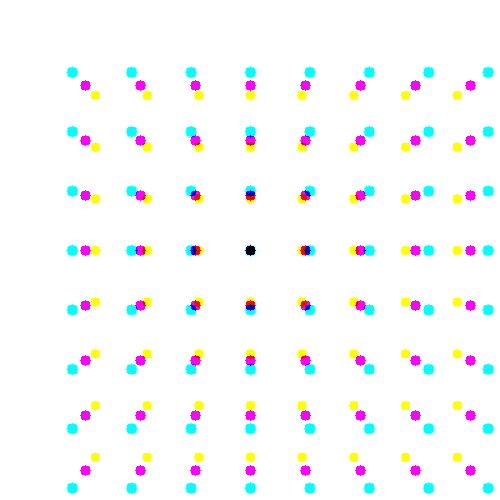
\includegraphics[width=0.48\textwidth]{figures/target.png}
\caption{Синтетическая точечная мишень с поперечной хроматической
аберрацией (R смещён на 8~\%, B — на 6~\%)}
\label{fig:target}
\end{figure}

\begin{figure}[H]
\centering
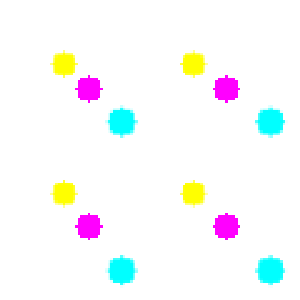
\includegraphics[width=0.45\textwidth]{figures/target_corner.png}
\caption{Увеличенный фрагмент угла мишени: цветные ореолы на контурах}
\label{fig:target_corner}
\end{figure}

В микроскопии калибровку хроматических аберраций традиционно выполняют с
помощью точечного препарата: микросфер (beads) или иного объекта с
заведомо малым размером. Такой препарат играет роль калибровочного кадра,
по которому измеряется смещение каналов~[8]. Разрабатываемое ПО реализует
именно такой режим калибровки, а также его слепой аналог.

\subsection{Математическая модель смещения}

Причиной поперечной аберрации является зависимость увеличения линзы от
длины волны. Первый член разложения этой зависимости по координате даёт
линейную зависимость смещения от радиуса, последующие — более высокие
степени. В общем случае радиальное смещение $d$ канала относительно
опорного на расстоянии $r$ от оптического центра описывается полиномом:
\begin{equation}
d(r) = c_1 r + c_2 r^2 + c_3 r^3,
\label{eq:poly}
\end{equation}
где $c_1$, $c_2$, $c_3$ — коэффициенты модели, подлежащие определению при
калибровке~[5, 7].

В слепом режиме, когда калибровочный кадр отсутствует и смещения
оцениваются по краям самого снимка, используется линейная модель:
\begin{equation}
d(r) = k r,
\label{eq:linear}
\end{equation}
где $k$ — коэффициент пропорциональности~[10]. Линейная модель грубее,
однако
полином высокого порядка, построенный по зашумлённым краям реального
снимка, при экстраполяции даёт неустойчивый результат; кроме того, как
показано в разделе~1.1, линейный член является доминирующим.

Измерение смещения канала по калибровочному кадру выполняется следующим
образом. Для каждой точки калибровочной мишени определяется её положение
в каждом цветовом канале, после чего вычисляется проекция вектора
смещения на радиальное направление:
\begin{equation}
d_i = (\mathbf{p}_{c,i} - \mathbf{p}_{g,i}) \cdot
      \frac{\mathbf{p}_{g,i} - \mathbf{p}_0}{\lVert \mathbf{p}_{g,i} -
      \mathbf{p}_0 \rVert},
\label{eq:proj}
\end{equation}
где $\mathbf{p}_{c,i}$ — положение $i$-й точки в измеряемом канале,
$\mathbf{p}_{g,i}$ — её положение в опорном (зелёном) канале, $\mathbf{p}_0$ —
оптический центр. Тем самым задача сводится к скалярным данным
$(r_i, d_i)$.

Коэффициенты модели \eqref{eq:poly} находятся методом наименьших
квадратов: минимизируется сумма квадратов невязок
\begin{equation}
S = \sum_i \Bigl(d_i - \sum_{j=1}^{3} c_j r_i^{j}\Bigr)^2
    \;\to\; \min_{c_1, c_2, c_3}.
\label{eq:lstsq}
\end{equation}
Задача \eqref{eq:lstsq} линейна относительно коэффициентов и решается
через нормальные уравнения.

Для оценки смещения по краям снимка (слепой режим) используются профили
яркости вдоль радиального направления. Смещение измеряется как аргумент
максимума нормированной взаимной корреляции профиля измеряемого канала с
профилем опорного:
\begin{equation}
\rho(s) = \frac{\sum_t \bigl(g(t) - \bar{g}\bigr)\bigl(c(t+s) -
\bar{c}_s\bigr)}
{\sqrt{\sum_t \bigl(g(t) - \bar{g}\bigr)^2 \sum_t
\bigl(c(t+s) - \bar{c}_s\bigr)^2}},
\label{eq:ncc}
\end{equation}
где $g(t)$ и $c(t)$ — отсчёты профилей опорного и измеряемого каналов,
$\bar{g}$ и $\bar{c}_s$ — их средние значения. Максимум дискретной
корреляции уточняется до субпиксельной точности параболической
интерполяцией трёх соседних отсчётов:
\begin{equation}
\hat{s} = s^{*} + \frac{1}{2}\cdot\frac{y_{-} - y_{+}}{y_{-} - 2M + y_{+}},
\label{eq:subpixel}
\end{equation}
где $M$ — значение корреляции в максимуме $s^{*}$, $y_{-}$ и $y_{+}$ — значения
корреляции в соседних отсчётах слева и справа.

\subsection{Обзор существующих решений}

Задача коррекции хроматических аберраций решается несколькими классами
программных средств. Сравнение представлено в таблице~1.

\begin{table}[H]
\caption{Обзор существующих средств коррекции хроматических аберраций}
\label{tab:compare}
\small
\begin{tabular}{|p{4.2cm}|p{4.4cm}|p{6.4cm}|}
\hline
Средство & Режим коррекции & Модель смещения \\
\hline
Adobe Lightroom Classic & профиль объектива или ручная правка & попиксельные ползунки, неявная модель по полю кадра \\
\hline
OpenCV 5.0 & по калибровочному кадру мишени & полином высокой степени (до 11-й), оценивается МНК [4] \\
\hline
Hugin (fulla) & по контрольным точкам & полиномиальная модель по радиусу \\
\hline
Разрабатываемое ПО & по калибровочному кадру и слепой (по снимку) & кубический полином \eqref{eq:poly} и линейная модель \eqref{eq:linear} \\
\hline
\end{tabular}
\end{table}

Фотографические редакторы (Lightroom, RawTherapee) применяют
профили объективов либо ручную коррекцию и ориентированы на
интерактивную работу, а не на автоматическую пакетную обработку
микрофотографий. Библиотека OpenCV предоставляет функцию
\texttt{correctChromaticAberration}, основанную на калибровке по кадру
мишени с полиномиальной моделью высокой степени [4]; это решение
универсально, но требует отдельного калибровочного кадра и не имеет
слепого режима. Разрабатываемое ПО сочетает оба режима и ориентировано
на работу с одиночным снимком в отсутствие калибровки.

\subsection{Выбор средств реализации}

В качестве языка реализации выбран Python~3 ввиду наличия зрелых
библиотек численных вычислений и обработки изображений. Для работы с
массивами используется NumPy~[6], для операций над изображениями
(свёртки, ремап, цветовые преобразования) — OpenCV~[4]. Графический
интерфейс реализован средствами штатной библиотеки
Tkinter, не требующей дополнительных зависимостей. Модульное тестирование
выполняется с помощью библиотеки pytest. Перечисленный набор
непротиворечив, свободно распространяется и полностью покрывает задачи
работы.

\clearpage
\section{Конструкторская часть}

\subsection{Требования к программному обеспечению}

К разрабатываемому ПО предъявляются следующие требования:
\begin{enumerate}
\item автоматическая коррекция поперечной хроматической аберрации без
ручного вмешательства пользователя;
\item возможность работы как по калибровочному кадру точечной мишени, так
и без него (слепой режим);
\item количественная оценка внесённой поправки и остаточного смещения
каналов;
\item загрузка исходного снимка через графический интерфейс и визуальное
сравнение результатов «до» и «после»;
\item сохранение результатов обработки на диск независимо от состояния
интерфейса;
\item работа с изображениями широкого диапазона разрешений
(от 0,3 до 12~Мпикс) без существенного роста времени обработки.
\end{enumerate}

\subsection{Архитектура программной системы}

Система построена по модульному принципу и разделена на вычислительное
ядро (пакет \texttt{achrom}) и графический интерфейс (\texttt{app.py}).
Ядро не зависит от интерфейса и может использоваться как библиотека.
Архитектура показана на рисунке~3.

\begin{figure}[H]
\centering
\resizebox{\linewidth}{!}{%
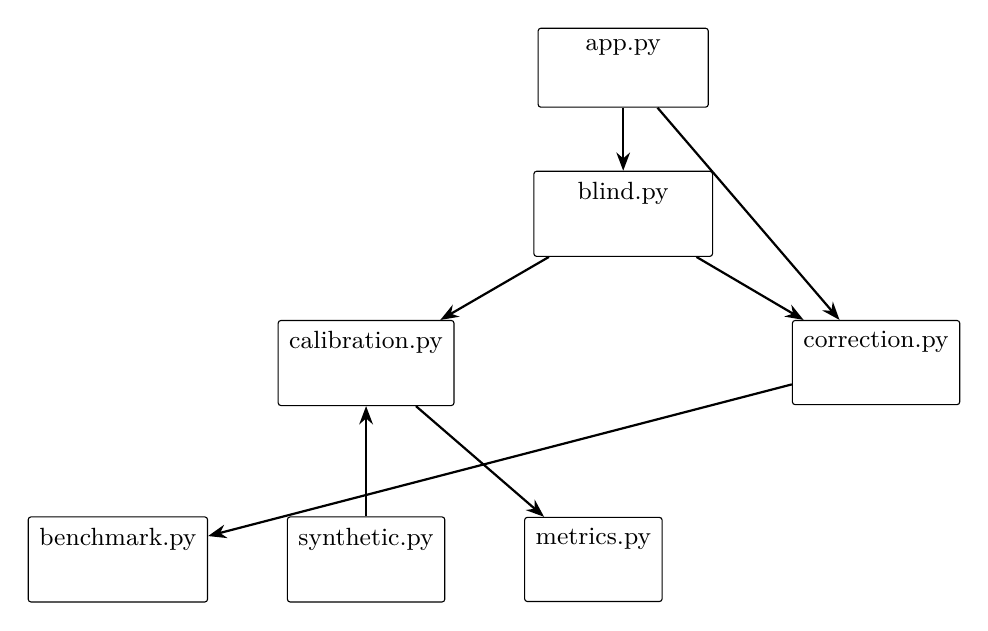
\begin{tikzpicture}[
  node distance=8mm and 10mm,
  box/.style={draw,rounded corners=1pt,align=center,inner sep=4pt,
              minimum height=9mm,font=\small},
  arr/.style={-{Stealth[]},thick}]
\node[box] (app) {app.py\\графический интерфейс};
\node[box,below=of app] (blind) {blind.py\\слепая оценка смещений};
\node[box,below left=of blind] (calib) {calibration.py\\подгонка и модель};
\node[box,below right=of blind] (corr) {correction.py\\обратный варп};
\node[box,below=14mm of calib] (synth) {synthetic.py\\генератор мишени};
\node[box,right=of synth] (metrics) {metrics.py\\оценка остатка};
\node[box,left=of synth] (bench) {benchmark.py\\замер времени};
\draw[arr] (app) -- (blind);
\draw[arr] (app) -- (corr);
\draw[arr] (blind) -- (calib);
\draw[arr] (blind) -- (corr);
\draw[arr] (calib) -- (metrics);
\draw[arr] (corr) -- (bench);
\draw[arr] (synth) -- (calib);
\end{tikzpicture}}
\caption{Архитектура программной системы}
\label{fig:arch}
\end{figure}

Модуль \texttt{calibration.py} выполняет обнаружение точек мишени,
измерение смещений \eqref{eq:proj} и подгонку модели \eqref{eq:poly}
методом наименьших квадратов, а также содержит функцию вычисления
полинома по коэффициентам. Модуль \texttt{correction.py} реализует
обратное радиальное смещение каналов. Модуль \texttt{blind.py} реализует
слепую оценку смещений по краям снимка. Вспомогательные модули
\texttt{synthetic.py}, \texttt{metrics.py} и \texttt{benchmark.py}
формируют тестовые данные, оценивают остаточное смещение и измеряют время
обработки соответственно.

\subsection{Калибровка объектива по калибровочному кадру}

Калибровка по кадру точечной мишени включает следующие этапы:
\begin{enumerate}
\item обнаружение точек (дисков) мишени в каждом цветовом канале;
\item определение положения каждой точки с субпиксельной точностью как
центра масс окрестности;
\item сопоставление точек между каналами и вычисление радиальных
смещений по формуле \eqref{eq:proj};
\item подгонка коэффициентов модели \eqref{eq:poly} методом наименьших
квадратов.
\end{enumerate}

Обнаружение дисков работает на обоих типах мишени (тёмные точки на светлом
фоне и светлые на тёмном) благодаря анализу знака локального контраста.
Качество коррекции количественно оценивается средним и максимальным
остаточным смещением каналов после её применения.

Проверка корректности калибровки выполнена на синтетическом кадре с
заведомо известными коэффициентами смещения (R~$+8~\%$, B~$-6~\%$).
После калибровки такие же коэффициенты были применены к другому кадру
с той же аберрацией, но иным расположением точек. Результат показан на
рисунке~4: среднее расхождение каналов уменьшилось с 11,92 до 0,83~пикс
(максимальное — с 24,88 до 1,80~пикс), то есть более чем на порядок.

\begin{figure}[H]
\centering
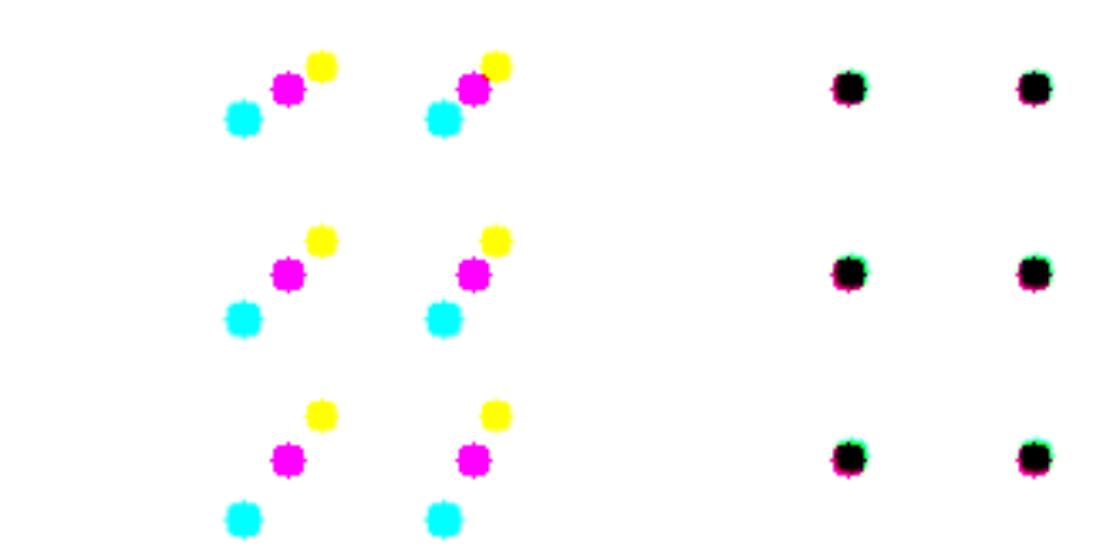
\includegraphics[width=0.85\textwidth]{figures/demo_diff.png}
\caption{Результат калиброванной коррекции синтетического кадра:
слева — до коррекции, справа — после}
\label{fig:demo}
\end{figure}

\subsection{Алгоритм обратной коррекции}

Коррекция состоит в обратном радиальном смещении красного и синего
каналов к опорному зелёному. Для каждого выходного пикселя на радиусе
$r$ требуется найти такой радиус $s$ во входном изображении, значение с
которого искажено меньше всего. Поскольку смещение задано в терминах
входного радиуса, искомый радиус $s$ является решением уравнения
фиксированной точки
\begin{equation}
s = r + d(s),
\label{eq:fixedpoint}
\end{equation}
которое находится методом последовательных приближений:
\begin{equation}
s^{(0)} = r, \qquad s^{(n+1)} = r + d\bigl(s^{(n)}\bigr).
\label{eq:iteration}
\end{equation}
Для используемых моделей смещения уравнение \eqref{eq:fixedpoint}
решается итерациями \eqref{eq:iteration}, которые сходятся
за несколько шагов. Пересчёт координат выполняется одним вызовом функции
ремапа для канала с билинейной интерполяцией; за границами кадра значения
продлеваются краевым пикселем, что предотвращает появление чёрной рамки.

\subsection{Слепой режим оценки смещений}

Слепой режим не требует калибровочного кадра и опирается на тот факт, что
контрастный край снимка присутствует во всех цветовых каналах
одинаково, а поперечная аберрация лишь растягивает каналы радиально.
Алгоритм состоит из следующих шагов:
\begin{enumerate}
\item по градиенту яркости зелёного канала отбираются точки краёв
(верхние 2~\% по величине градиента), при этом исключаются точки вблизи
центра и на границе кадра, а также точки, край которых не перпендикулярен
радиальному направлению;
\item через каждую отобранную точку строится профиль яркости вдоль
радиуса (окно $\pm28$~пикс) для каждого канала;
\item смещение измеряется как аргумент максимума корреляции \eqref{eq:ncc}
с субпиксельным уточнением \eqref{eq:subpixel}; пары с низкой корреляцией
($<0{,}75$) отбрасываются;
\item по данным $(r_i, d_i)$ подгоняется линейная модель \eqref{eq:linear};
выбросы с остатком более 1~пикс отбрасываются, подгонка повторяется;
\item найденные коэффициенты применяются функцией коррекции, после чего
оценка повторяется по скорректированному изображению. Итерации
прекращаются, когда остаточное смещение становится менее 0,5~пикс
(но не более трёх итераций).
\end{enumerate}

Итеративная схема необходима потому, что смещение измеряется по уже
отчасти исправленному изображению: каждая следующая итерация уточняет
коэффициенты и уменьшает остаток.

\subsection{Графический интерфейс}

Интерфейс реализует основной сценарий работы: пользователь нажимает
кнопку «Загрузить снимок», выбирает файл изображения, после чего
выполняется слепая автокоррекция. Обработка идёт в фоновом потоке, поэтому
окно интерфейса не замораживается. Обновление элементов интерфейса
производится исключительно из главного потока опросом состояния задачи
через механизм отложенных вызовов Tkinter, поскольку библиотека Tkinter
не допускает обращений из других потоков.

По завершении обработки в подкаталог \texttt{results} записываются три
файла: изображение до коррекции, изображение после коррекции и парное
изображение для сравнения (увеличенные фрагменты наиболее удалённого от
центра угла кадра, где аберрация максимальна). Файлы сохраняются на диск
до отображения, поэтому результат не теряется даже при закрытии окна во
время обработки. Парное изображение открывается в системном просмотрщике
изображений. Все исключения протоколируются в журнале \texttt{app.log}.

Режим калибровки по точечному кадру реализован как программный интерфейс
библиотеки и продемонстрирован в разделе~4; графический интерфейс
ориентирован на типовой сценарий обработки одиночного снимка.

\clearpage
\section{Технологическая часть}

\subsection{Технологический стек}

Программное обеспечение реализовано на языке Python~3.9. Для численных
вычислений используются библиотеки NumPy~2.0 и OpenCV~5.0, для работы с
изображениями при сохранении — OpenCV и Pillow. Графический интерфейс
построен на штатной библиотеке Tkinter. Тестирование выполняется
библиотекой pytest. Все зависимости свободно распространяются.

\subsection{Организация исходного кода}

Исходный код разделён на пакет вычислительного ядра \texttt{achrom} и
головной модуль \texttt{app.py}. Пакет содержит модули
\texttt{calibration}, \texttt{correction}, \texttt{blind},
\texttt{synthetic}, \texttt{metrics}, \texttt{benchmark} в соответствии с
архитектурой (рисунок~\ref{fig:arch}). Полные листинги модулей приведены в
приложениях~А–Г.

\subsection{Модульное тестирование}

Разработка велась по методике тестирования на основе спецификации:
для каждой функции сначала создавался тест, затем реализация. Ожидаемые
значения в тестах берутся из независимого источника — известных
коэффициентов генератора синтетических изображений или ручного расчёта,
а не из повторного применения проверяемого алгоритма. Всего реализовано
13~тестов, покрывающих:
\begin{itemize}
\item обнаружение точек мишени на светлом и тёмном фоне;
\item измерение смещений на кадре с известным коэффициентом;
\item восстановление полиномиальной модели по синтетическим данным;
\item коррекцию кадра, не входившего в обучающую выборку;
\item слепую оценку смещения на синтетическом кадре с известным
коэффициентом;
\item отсутствие ложной коррекции при нулевой аберрации;
\item работу интерфейса коррекции во всём диапазоне разрешений и замер
времени.
\end{itemize}

\clearpage
\section{Аналитическая часть}

\subsection{Тестовые данные}

Исследование проводилось на синтетических кадрах с известной аберрацией и
на реальных снимках, содержащих выраженную поперечную хроматическую
аберрацию. Поскольку открытые микрофотографии с известными параметрами
аберрации в свободном доступе отсутствуют, в качестве реальных данных
использованы снимки с аналогичным характером искажений: макросъёмка и
кадры, снятые объективами без хроматической коррекции. Синтетические
кадры имитируют калибровочный препарат микроскопа. Характеристики
тестовых изображений приведены в таблице~2.

\begin{table}[H]
\caption{Характеристики тестовых изображений}
\label{tab:data}
\small
\begin{tabular}{|p{3.2cm}|p{5.2cm}|p{2.2cm}|p{4cm}|}
\hline
Файл & Описание & Разрешение & Смещение R / B, первый проход \\
\hline
real\_macro\_ca.jpg & макросъёмка, Canon PowerShot & 5184$\times$2912 & $-8{,}7$ / $+10{,}9$ \\
\hline
lens\_ca.jpg & кадр с аберрацией объектива & 2462$\times$2532 & $-8{,}1$ / $+14{,}0$ \\
\hline
holga\_tatra.jpg & съёмка камерой Holga & 3840$\times$2566 & $-2{,}2$ / $+2{,}7$ \\
\hline
detail\_ca.jpg & кадр с умеренной аберрацией & 2592$\times$2592 & $-1{,}0$ / $+2{,}1$ \\
\hline
real\_blende8.jpg & контрольный кадр без аберрации & 2000$\times$1328 & $-0{,}1$ / $+0{,}2$ \\
\hline
\end{tabular}
\end{table}

Изображения заимствованы из открытого архива Wikimedia Commons под
свободными лицензиями (CC0, CC~BY-SA~3.0, CC~BY-SA~4.0). Последнее
изображение является контрольным: оно снято камерой с внутрикамерной
коррекцией и не содержит заметной аберрации.

\subsection{Результаты коррекции}

Слепая коррекция выполнена для каждого изображения. Суммарная внесённая
поправка, остаточное смещение (по результатам финальной оценки) и число
выполненных итераций приведены в таблице~3.

\begin{table}[H]
\caption{Результаты слепой коррекции}
\label{tab:results}
\small
\begin{tabular}{|p{3.2cm}|p{3cm}|p{3.4cm}|p{2.1cm}|p{1.8cm}|}
\hline
Изображение & Суммарная поправка R / B, пикс & Остаток R / B, пикс & Итераций & Время, с \\
\hline
real\_macro\_ca.jpg & $-9{,}7$ / $+15{,}6$ & $-0{,}4$ / $+0{,}7$ & 3 & 2,0 \\
\hline
lens\_ca.jpg & $-8{,}2$ / $+14{,}7$ & $-0{,}0$ / $+0{,}1$ & 2 & 0,7 \\
\hline
holga\_tatra.jpg & $-2{,}2$ / $+2{,}7$ & $-0{,}1$ / $+0{,}2$ & 1 & 0,6 \\
\hline
detail\_ca.jpg & $-1{,}0$ / $+2{,}1$ & $-0{,}3$ / $+0{,}3$ & 1 & 0,3 \\
\hline
real\_blende8.jpg & — & — & 0 & $<$0,1 \\
\hline
\end{tabular}
\end{table}

Во всех случаях с выраженной аберрацией остаточное смещение после
коррекции снизилось до долей пикселя (менее 0,7~пикс), что соответствует
погрешности измерения. Для контрольного изображения без аберрации
оценённое смещение не превысило порога 0,5~пикс, и коррекция не
выполнялась — это подтверждает отсутствие ложных срабатываний.

На рисунке~5 показан результат для макросъёмки с наибольшим смещением,
на рисунке~6 — для кадра с аберрацией объектива. На обоих фрагментах видно
устранение цветных ореолов на контурах.

\begin{figure}[H]
\centering
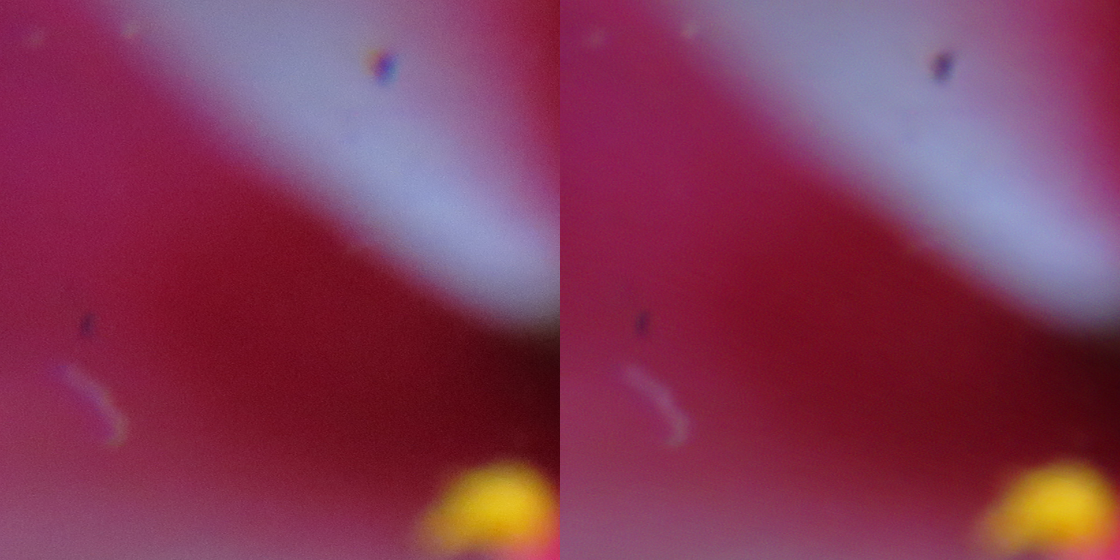
\includegraphics[width=0.9\textwidth]{figures/macro_diff.png}
\caption{Макросъёмка с выраженной поперечной аберрацией
(R $-9{,}7$~пикс, B $+15{,}6$~пикс): слева — до, справа — после}
\label{fig:macro}
\end{figure}

\begin{figure}[H]
\centering
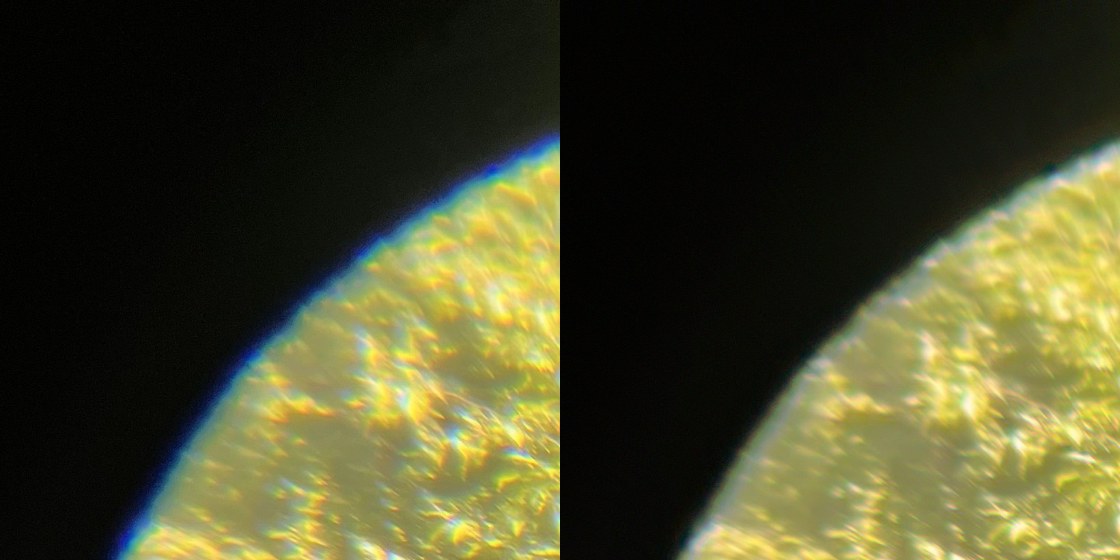
\includegraphics[width=0.9\textwidth]{figures/lens_diff.png}
\caption{Кадр с хроматической аберрацией объектива
(R $-8{,}1$~пикс, B $+14{,}0$~пикс): слева — до, справа — после}
\label{fig:lens}
\end{figure}



Отдельно исследован случай продольной хроматической аберрации, при
которой цветовые каналы различаются степенью размытия, а не радиальным
смещением. Слепой алгоритм в этом случае не обнаруживает значимого
смещения и не вносит коррекции, что согласуется с теоретической моделью:
продольная аберрация не описывается радиальным растяжением каналов и
требует других методов (например, деконволюции с разными ядрами для
каналов).

\subsection{Зависимость времени обработки от разрешения}

Время коррекции измерено для изображений от 0,3 до 12~Мпикс. Результаты
приведены в таблице~4 и на рисунке~8.

\begin{table}[H]
\caption{Время коррекции в зависимости от разрешения}
\label{tab:time}
\small
\begin{tabular}{|p{2.6cm}|p{2.4cm}|p{2.6cm}|p{3.2cm}|}
\hline
Разрешение & Пикселей, Мпикс & Время, мс & Удельно, мс/Мпикс \\
\hline
640$\times$480 & 0,31 & 24,5 & 79,8 \\
\hline
1280$\times$960 & 1,23 & 64,8 & 52,7 \\
\hline
1920$\times$1440 & 2,76 & 147,3 & 53,4 \\
\hline
2560$\times$1920 & 4,92 & 254,4 & 51,7 \\
\hline
3840$\times$2880 & 11,06 & 614,1 & 55,5 \\
\hline
\end{tabular}
\end{table}

\begin{figure}[H]
\centering
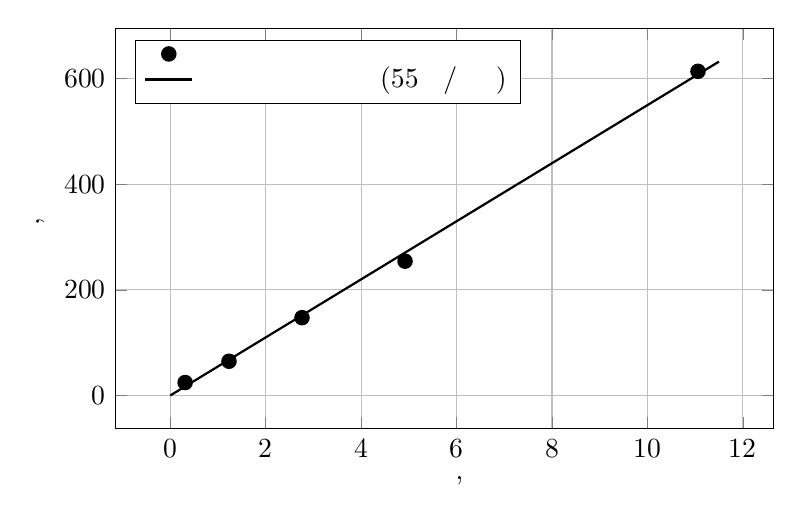
\begin{tikzpicture}
\begin{axis}[
  width=0.82\textwidth,
  height=0.55\textwidth,
  xlabel={Разрешение, Мпикс},
  ylabel={Время, мс},
  grid=major,
  legend pos=north west,
  legend cell align=left,
  every axis plot/.append style={thick},
]
\addplot[only marks,mark=*,mark size=2.4pt] coordinates
  {(0.31,24.5)(1.23,64.8)(2.76,147.3)(4.92,254.4)(11.06,614.1)};
\addplot[domain=0:11.5] {55*x};
\legend{измерения, линейная аппроксимация (55~мс/Мпикс)}
\end{axis}
\end{tikzpicture}
\caption{Зависимость времени коррекции от разрешения изображения}
\label{fig:time}
\end{figure}

Время обработки возрастает практически линейно с числом пикселей;
удельные затраты составляют около 55~мс на мегапиксель. Наименьшее
разрешение имеет повышенные удельные затраты (80~мс/Мпикс) из-за
постоянных накладных расходов, которые при больших разрешениях становятся
пренебрежимо малы. Таким образом, время обработки снимка типовой
микрофотографии (несколько мегапикселей) составляет доли секунды, что
приемлемо для практического применения.

\structural{ЗАКЛЮЧЕНИЕ}

В ходе курсовой работы разработано программное обеспечение для
автоматической коррекции поперечной хроматической аберрации
микрофотографий. Получены следующие результаты.

Исследована природа хроматических аберраций и построена математическая
модель поперечной аберрации в виде радиального полинома, учитывающая
доминирующий линейный член и нелинейные поправки.

Реализована калибровка объектива по точечному калибровочному кадру с
количественной оценкой остаточных смещений. На синтетическом кадре с
известной аберрацией среднее расхождение каналов уменьшилось с 11,92 до
0,83~пикс (более чем на порядок).

Реализован слепой режим оценки смещений по самому снимку, не требующий
калибровочного кадра. На реальных изображениях с аберрацией остаточное
смещение после коррекции снизилось до долей пикселя; при этом алгоритм не
вносит ложной коррекции при отсутствии аберрации.

Разработан графический интерфейс с загрузкой снимка и визуальным
сравнением результатов «до/после»; обработка идёт в фоновом потоке,
результаты сохраняются на диск независимо от состояния окна.

Исследована зависимость времени обработки от разрешения: время растёт
линейно и составляет около 55~мс на мегапиксель.

В качестве ограничений отмечено, что продольная хроматическая аберрация
не описывается радиальной моделью смещения и не корректируется
разработанными средствами. Направлениями дальнейшей работы являются
коррекция продольной аберрации методами деконволюции, автоматическое
определение оптического центра и распараллеливание вычислений
на графическом процессоре.

\structural{СПИСОК ИСПОЛЬЗОВАННЫХ ИСТОЧНИКОВ}

\begin{enumerate}
\item 1. Гонсалес Р., Вудс Р. Цифровая обработка изображений. — 3-е изд.,
испр. и доп. — М.: Техносфера, 2012. — 1104~с.
\item Прэтт У. Цифровая обработка изображений: в 2 кн. — М.: Мир, 1982. —
Кн.~1. — 312~с.; кн.~2. — 480~с.
\item Яне Б. Цифровая обработка изображений. — М.: Техносфера, 2007. —
584~с.
\item Bradski G. The OpenCV Library // Dr. Dobb's Journal of Software
Tools. — 2000. — Vol.~25, no.~11. — P.~120–125.
\item Brown D. C. Decentering distortion of lenses // Photogrammetric
Engineering. — 1966. — Vol.~32, no.~3. — P.~444–462.
\item Harris C. R. et al. Array programming with NumPy // Nature. —
2020. — Vol.~585. — P.~357–362.
\item Hartley R., Zisserman A. Multiple View Geometry in Computer
Vision. — 2nd ed. — Cambridge: Cambridge University Press, 2004. —
655~p.
\item Leiwe M. N., Fujimoto S., Imai T. Post hoc correction of chromatic
aberrations in large-scale volumetric images in confocal microscopy //
Frontiers in Neuroanatomy. — 2021. — Vol.~15. — Art.~760063.
\item Szeliski R. Computer Vision: Algorithms and Applications. —
2nd ed. — Cham: Springer, 2022. — 925~p.
\item Zhang Z. A Flexible New Technique for Camera Calibration //
IEEE Transactions on Pattern Analysis and Machine Intelligence. — 2000. —
Vol.~22, no.~11. — P.~1330–1334.
\end{enumerate}

\apphead{А}{Модули калибровки и формирования тестовых данных}
\lstinputlisting[caption={Модуль calibration.py}]{src/calibration.py}
\lstinputlisting[caption={Модуль synthetic.py}]{src/synthetic.py}
\lstinputlisting[caption={Модуль metrics.py}]{src/metrics.py}

\apphead{Б}{Модули коррекции и замера времени}
\lstinputlisting[caption={Модуль correction.py}]{src/correction.py}
\lstinputlisting[caption={Модуль benchmark.py}]{src/benchmark.py}

\apphead{В}{Модуль слепой оценки смещений}
\lstinputlisting[caption={Модуль blind.py}]{src/blind.py}

\apphead{Г}{Графический интерфейс}
\lstinputlisting[caption={Модуль app.py}]{src/app.py}

\end{document}
